\section{Statistics}

\subsection{Correlation}
Assume an inner product space.

\subsection{Linear regression}

Assume that reality can me modelled by a model like this one: 

$$ \vec{y} = \mtrx{X} \vec{w} + \vec{e} $$

Not knowing $\vec{e}$, our best guess at the outcome would be 

$$ \vec{\hat{y}} = \mtrx{X} \vec{w} $$

We can find the gradient of w by:

$$ \partDiff{E}{\vec{w}} = -  (\vec{y} - \vec{\hat{y}}) \mtrx{X}  $$





\subsubsection{You are absolutely allowed to invert a linear regression relation}
Linear regressions are focussed on $P(y | x)$ ... but you can absolutely revert that relation. For example, you are allowed to predict size from basketball scores, even though in reality it's likely the other way round.

Assume 
$$ y = \alpha x + \epsilon $$
and 
$$ \epsilon ~ N(0, \sigma^2_\epsilon), x ~ N(\mu_x, \sigma^2_x)$$
This yields $P(y|x) = N(\alpha x, \sigma^2_\epsilon)$. But in the same vain we may also write
$$ x = \frac{y}{\alpha} - \frac{\epsilon}{\alpha} $$
With:
$$ P(x|y) = N(\frac{\mu_y}{\alpha},  \frac{\sigma^2_\epsilon}{\alpha^2}) $$

We can also arrive at the same joint distribution $P(x, y)$ coming from $x$ as well as from $y$.

\begin{equation}
    \begin{aligned}
        P(x, y) &= P(y|x) P(x) &= N(\alpha x, \sigma^2_\epsilon) N(\mu_x, \sigma^2_x) \\
                &= P(x|y) P(y) &= N( \frac{y}{\alpha}, \frac{\sigma^2_\epsilon}{\alpha^2} ) \int_X P(x, y)
    \end{aligned}
\end{equation}

All the regression-model tells us, is that there is a relation $ y = \alpha x + \epsilon $ between $x$ and $y$. It does \emph{not} imply a direction or causality.

\subsection{Spatial modelling}

\subsubsection{Generalized least squares}
like linear regression, but errors are not iid, but allowed to be correlated.

\subsubsection{Gaussian processes}
Gaussian processes are a means of interpolating a value $y_x$ from surrounding values $y_x = \sum \alpha_i y_i$. Basic intuition from \href{https://bookdown.org/rbg/surrogates/chap5.html}{here}.
That is different from what linear regression or its extension GLS do: regression predicts $y$ from explanatory variables $x$, assuming a (linear) model.
Gaussian processes don't do that. They only interpolate between already observed $y$'s. No model is assumed.

Consider the $n \times m$ surface $\mtrx{Y}$. Assume that the value of any pixel in $\mtrx{Y}$ follows a gaussian distribution - which may be correlated to all other pixels in $\mtrx{Y}$.
Millions of surfaces $\mtrx{Y}$ may be sampled from $N(\vec{0}, \mtrx{\Sigma}) = P(\mtrx{Y})$, where $\vec(0)$ is of size $n \times m$ and $\mtrx{\Sigma}$ is of size $nm \times nm$.
We call $P(\mtrx{Y})$ the prior. $\mtrx{\Sigma}$ can be very large, so we assume that it can be modeled by a covariance-function $cov(h)$ which is \emph{only dependent on the distance between two points, not on the points themselves}.

\begin{lstlisting}[language=python]
import numpy as np
import matplotlib.pyplot as plt
from scipy.stats import multivariate_normal


NOISEFACTOR = 0.001


def size(x):
    return np.sqrt(np.sum(np.power(x, 2)))

def distance(x0, x1):
    return size(x0 - x1)

def getDistanceMatrix(rowPoints, colPoints):
    # deliberately not exploiting symmetry 
    # <- this way it works with non-square matrices, too.
    rows = len(rowPoints)
    cols = len(colPoints)
    distances = np.zeros((rows, cols))
    for i in range(rows):
        for j in range(cols): 
            p0 = rowPoints[i]
            p1 = colPoints[j]
            d = distance(p0, p1)
            distances[i, j] = d
    return distances

deltaX = 0.1
deltaY = 0.1
gridX = 40
gridY = 60
nrPoints = gridX * gridY
points = np.zeros((nrPoints, 2))
i = 0
for x in range(gridX):
    for y in range(gridY):
        points[i] = [x * deltaX, y * deltaY]
        i += 1
distances = getDistanceMatrix(points, points)

mean = np.zeros((nrPoints))
cov0 = 2.3  # variance without distance: Cov(0) = Cov(Z(x), Z(x)) = Var(Z | x)
h95 = 40     # distance at which cov(h) >= 0.95 * cov0

def variogramFunction(h):
    return cov0 * ( 1 - np.exp( -3*h/h95 ) )

Sigma = cov0 - variogramFunction(distances)
Sigma += NOISEFACTOR * np.eye(nrPoints) * np.random.rand(nrPoints) # to make inverse possible
prior = multivariate_normal(mean, Sigma, allow_singular=True)

sample1 = prior.rvs()
sample2 = prior.rvs()
sample3 = prior.rvs()
\end{lstlisting}

\begin{figure}[H]
    \caption{3 samples from prior $P(\mtrx{Y})$}
    \centering
    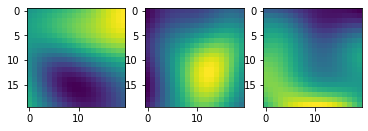
\includegraphics[width=0.7\linewidth]{images/gp_prior_samples.png}
\end{figure}

We have observed some samples $\mtrx{D} = {(x_i, y_i)}$.
Which of these millions of surfaces are most likely given those observations? We can answer that with $P(\mtrx{Y}|\mtrx{D})$.
\begin{figure}[H]
    \caption{Observations $\mtrx{D}$. Which field $\mtrx{Y}$ is most likely to have produced these observations?}
    \centering
    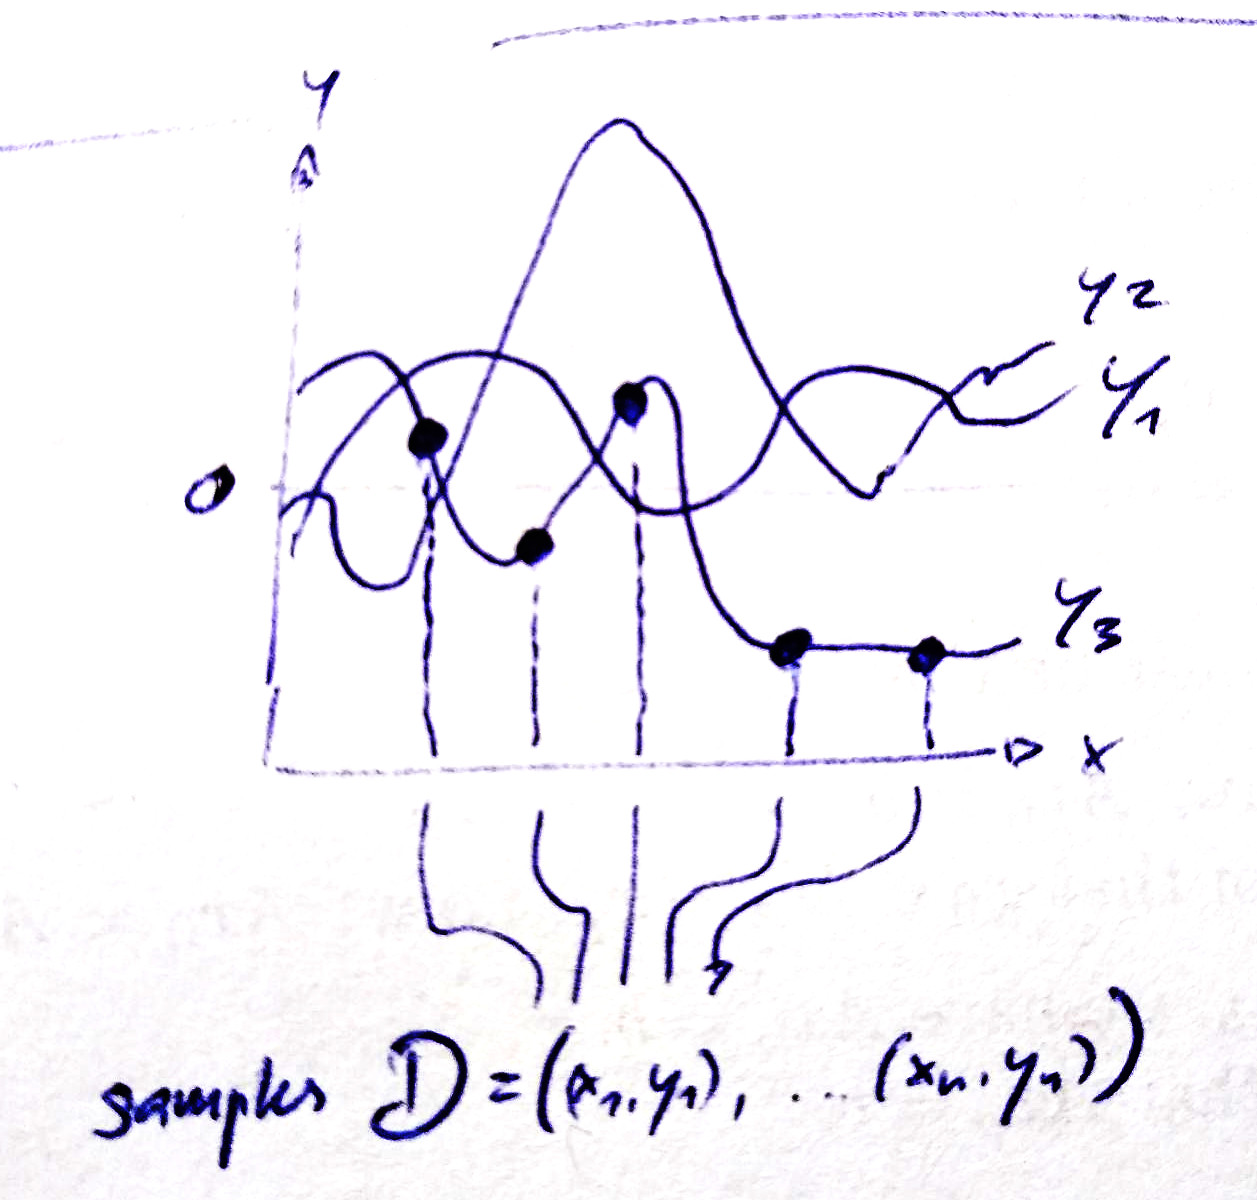
\includegraphics[width=0.4\linewidth]{images/gp_observations.jpg}
\end{figure}

We can calculate the posterior using 
$$
P(\mtrx{Y}|\mtrx{D}) \sim P(\mtrx{D}|\mtrx{Y}) P(\mtrx{Y})
$$
But since in gaussian processes we assume multivariate-normals, this can be done much easier.

Consider a multivariate normal distribution on, say, 400 dimensions $N(\vec{\mu}, \mtrx{\Sigma})$. Those 400 dimensions could, for example, be pixel-values in a 20 by 20 image.
Now assume that out of those 400 dimensions we have measurements for $s$ samples, leaving a rest $r = 400 - s$.
For multivariate-normal distributions, we can easily and analytically obtain the conditional distribution $P(\vec{y}_r | \vec{y}_s) = N(\hat{\vec{\mu}}, \hat{\mtrx{\Sigma}})$.

Split $\vec{y}$ like so:
$$ y = \myarray{\vec{y}_r \\ \vec{y}_s} $$
Analogously we can split the covariance-matrix:
$$ \mtrx{\Sigma} = \begin{bmatrix}
    \mtrx{\Sigma}_{rr} & \mtrx{\Sigma}_{rs} \\
    \mtrx{\Sigma}_{sr} & \mtrx{\Sigma}_{ss} \\
\end{bmatrix}  $$

Then, according to \href{https://en.wikipedia.org/wiki/Multivariate_normal_distribution#Conditional_distributions}{wikipedia}, we can obtain $\hat{\vec{\mu}}$ and $\hat{\mtrx{\Sigma}}$ like so:
$$ \hat{\vec{\mu}}_r = \vec{\mu}_r + \mtrx{\Sigma}_{rs} \mtrx{\Sigma}_{ss}^{-1} (\vec{y}_s - \vec{\mu}_s) $$
$$ \hat{\mtrx{\Sigma}}_r = \mtrx{\Sigma}_{rr} - \mtrx{\Sigma}_{rs} \mtrx{\Sigma}_{ss}^{-1} \mtrx{\Sigma}_{sr} $$

\begin{lstlisting}[language=python]
indices = np.arange(nrPoints)
sampleIndices = np.asarray([13, 25, 84, 96]) # ... from data ...
sampleValues = np.asarray([4.6, 19, 9.4, 21]) # ... from data ...
samplePoints = points[sampleIndices]
nonSampleIndices = np.asarray(
        [i for i in indices 
            if i not in sampleIndices]
)
nonSamplePoints = points[nonSampleIndices]

# For simplicity, we just re-calculate SigmaXX here.
# But we could have also picked the right values from Sigma
# without any need for re-computation.
distancesRR = getDistanceMatrix(nonSamplePoints, nonSamplePoints)
SigmaRR = cov0 - variogramFunction(distancesRR)

distancesSS = getDistanceMatrix(samplePoints, samplePoints)
SigmaSS = cov0 - variogramFunction(distancesSS)
SigmaSS += NOISEFACTOR * np.eye(nrSamples) * np.random.rand(nrSamples) # To make inverse possible
SigmaSSInverse = np.linalg.inv(SigmaSS)

distancesRS = getDistanceMatrix(nonSamplePoints, samplePoints)
SigmaRS = cov0 - variogramFunction(distancesRS)
SigmaSR = SigmaRS.transpose()

meanPosterior = SigmaRS @ SigmaSSInverse @ sampleValues
SigmaPosterior = SigmaRR - SigmaRS @ SigmaSSInverse @ SigmaSR
SigmaPosterior += NOISEFACTOR * np.eye(nrPoints - nrSamples) * np.random.rand(nrPoints - nrSamples)  # To make inverse possible

posterior = multivariate_normal(meanPosterior, SigmaPosterior)   
\end{lstlisting}

We can now plot the \inlinecode{meanPosterior} around our \inlinecode{samples}. Doing so we obtain the graphic as shown in figure \ref{gpPosterior}.

\begin{figure}[H]
  \centering
  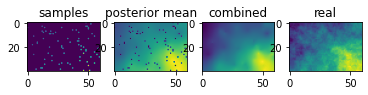
\includegraphics[width=0.7\linewidth]{images/gp_posterior_samples.png}
  \caption{Samples and fitted posterior fit together well}
  \label{gpPosterior}
\end{figure}


Note how we assumed that the covariance matrix $\mtrx{\Sigma}$ could be parameterized with a covariance-function $c(h)$. Only this way do we have any chance of finding a good approximation for $\mtrx{\Sigma}$ with only few samples.
The relation \inlinecode{Sigma = cov0 - variogramFunction(distances)} comes from the variogram $\gamma(h)$ as in here:
\begin{equation}
  \begin{aligned}
    2 \gamma(h) &= E[(Z(x+h) - Z(x))^2] \\
                &= E[( (Z(x+h) - \mu) - (Z(x) - \mu) )^2] \\
                &= E[ (Z(x+h) - \mu)^2  - 2(Z(x+h) - \mu)(Z(x) - \mu)  + (Z(x) - \mu)^2 ] \\
                &= E[ (Z(x+h) - \mu)^2 ]  - 2 E[(Z(x+h) - \mu)(Z(x) - \mu)]  + E[ (Z(x) - \mu)^2 ] \\
                &= c(0) - 2 c(h) + c(0) \\
      \gamma(h) &= c(0) - c(h) \\
           c(h) &= c(0) - \gamma(h)
  \end{aligned}
\end{equation}
In practical applications, we'll usually fit our function \inlinecode{cov0 * ( 1 - np.exp( -3*h/h95 ) )} by moving the parameters \inlinecode{cov0} and \inlinecode{h95} until the residuals fit properly.
Our code would then look like this:

\begin{lstlisting}[language=python]
def empiricalVariogram(distanceMatrix, data):
  variogram = {}
  d0 = np.min(distanceMatrix)
  d1 = np.max(distanceMatrix)
  nrHs = 20
  deltaH = (d1 - d0) / nrHs
  for h in np.linspace(d0, d1, nrHs):
      Nh = 0
      hSum = 0
      pairs = (h <= distanceMatrix) * (distanceMatrix < h+deltaH)
      for i in range(nrTotal):
          for j in range(i, nrTotal):
              if pairs[i, j]:
                  v = data[i]
                  vh = data[j]
                  hSum += np.power(v - vh, 2)
                  Nh += 1
      if Nh > 0:
          variogram[h] = hSum / (2 * Nh)
    return variogram
    
def fitVariogram(samples):
    pass  # TBD


residuals = prediction - samples
(cov0, h95) = fitVariogram(residuals)

SigmaRR = cov0 - variogramFunction(cov0, h95, distancesRR)
SigmaSS = cov0 - variogramFunction(cov0, h95, distancesSS)
SigmaRS = cov0 - variogramFunction(cov0, h95, distancesRS)
SigmaSR = SigmaRS.transpose()
SigmaSSInverse = np.linalg.inv(SigmaSS)

meanPosterior = prediction + SigmaRS @ SigmaSSInverse @ sampleValues
SigmaPosterior = SigmaRR - SigmaRS @ SigmaSSInverse @ SigmaSR

predictionPosterior = meanPosterior
\end{lstlisting}


For more, see this \href{https://michaeloneill.github.io/GPR-tutorial.html}{very thorough tutorial}.

\subsubsection{AR and SAR}
Autoregressive and spatial-autoregressive models.

\subsubsection{Comparison}

\begin{table}[H]
    \centering
    \resizebox{\textwidth}{!}{%
    \begin{tabular}{@{}llll@{}}
    \toprule
     &
      Generalized least squares &
      Gaussian processes &
      AR \\ \midrule
    \multicolumn{1}{|l|}{type} &
      \multicolumn{1}{l|}{\begin{tabular}[c]{@{}l@{}}Predict y from x.\\ Has explanatory variables.\end{tabular}} &
      \multicolumn{1}{l|}{\begin{tabular}[c]{@{}l@{}}Interpolate y from other y's.\\ Explanatories can be added with GLS\end{tabular}} &
      \multicolumn{1}{l|}{interpolate y from other y's} \\ \midrule
    \multicolumn{1}{|l|}{model} &
      \multicolumn{1}{l|}{\begin{tabular}[c]{@{}l@{}}$y = X\alpha + \epsilon$\\ \\ $\epsilon \sim N(\vec{0}, \mtrx{\Sigma})$\end{tabular}} &
      \multicolumn{1}{l|}{\begin{tabular}[c]{@{}l@{}}$Y \sim N(\vec{0}, \mtrx{\Sigma})$\\ $P(\mtrx{Y}|\mtrx{D}) = N(\hat{\vec{\mu}}, \hat{\mtrx{\Sigma}})$\\ $\tilde{y} = \sum \alpha_i \vec{y}_i$\\ Y is a field of size n by m\\ D is the observations \end{tabular}} &
      \multicolumn{1}{l|}{\begin{tabular}[c]{@{}l@{}}$y_t = \sum \alpha_i y_{t-i} + \epsilon$\\ $\epsilon \sim N(0, \sigma)$, iid \end{tabular}} \\ \midrule
    \multicolumn{1}{|l|}{Specialities} &
      \multicolumn{1}{l|}{} &
      \multicolumn{1}{l|}{\begin{tabular}[c]{@{}l@{}}$\mtrx{\Sigma}$ is encoded using a covariance-function cov(h)\\ to save on parameters\end{tabular}} &
      \multicolumn{1}{l|}{} \\ \midrule
    \multicolumn{1}{|l|}{$\epsilon$} &
      \multicolumn{1}{l|}{} &
      \multicolumn{1}{l|}{} &
      \multicolumn{1}{l|}{} \\ \midrule
    \multicolumn{1}{|l|}{$cov(\epsilon_i, \epsilon_j)$} &
      \multicolumn{1}{l|}{} &
      \multicolumn{1}{l|}{} &
      \multicolumn{1}{l|}{} \\ \midrule
    \multicolumn{1}{l|}{$cov(y_i, y_j)$} &
      \multicolumn{1}{l|}{} &
      \multicolumn{1}{l|}{} &
      \multicolumn{1}{l|}{} \\ \bottomrule
    \end{tabular}%
    }
    \end{table}


\subsection{Bayesian networks}
Bayesian networks are a neat tool when we can manually encode some complex causation-graphs.

\begin{lstlisting}[language=python]

  def find(lst, predicate):
  for entry in lst:
      if predicate(entry):
          return entry

def prod(lst):
  p = lst[0]
  for entry in lst[1:]:
      p *= entry
  return p

def getCombinations(lists):
  combinations = []
  if len(lists) == 0:
      combinations = []
  elif len(lists) == 1:
      combinations = lists[0]
  elif len(lists) == 2:
      for a in lists[0]:
          for b in lists[1]:
              combinations.append([a, b])
  else:
      firstList = lists[0]
      subCombos = getCombinations(lists[1:])
      for a in firstList:
          for b in subCombos:
              combinations.append([a, *b])
  return combinations



class Node:
  def __init__(self, name, pmf, allowedValues, parents = []):
      self.name = name
      self.pmf = pmf
      self.allowedValues = allowedValues
      self.parents = parents

  def setPmf(self, pmf):
      self.pmf = pmf

  def calcProb(self, value):

      if value not in self.allowedValues:
          return 0.0

      parentData = self.__getParentData()
      
      p = 0.0
      if len(parentData) > 0:
          for combination in getCombinations(parentData):
              parentValues = {entry['name']: entry['value'] for entry in combination}
              parentProbs = [entry['prob'] for entry in combination]
              p += self.pmf(value, parentValues) * prod(parentProbs)
      else:
          p = self.pmf(value, {})

      return p

  def __getParentData(self):
      parentData = []
      for i, parent in enumerate(self.parents):
          parentData.append([])
          for value in parent.allowedValues:
              prob = parent.calcProb(value)
              parentData[i].append({
                  'name': parent.name,
                  'value': value,
                  'prob': prob
              })
      return parentData


class Net:
  def __init__(self, nodes):
      self.nodes = nodes
      self.memo = {}
      for node in self.nodes:
          self.memo[node.name] = {}

  def calcProb(self, nodeName, value):
      if self.memo[nodeName][value]:
          return self.memo[nodeName][value]
      else:
          node = self.__findNode(nodeName)
          prob = node.calcProb(value)
          self.memo[nodeName][value] = prob
          return prob

  def setPmf(self, nodeName, pmf):
      # setting pmf
      node = self.__findNode(nodeName)
      node.setPmf(pmf)

      # invalidating downstream cached results
      self.memo[nodeName] = {}
      children = self.__findChildren(nodeName, True)
      for child in children:
          self.memo[child.name] = {}

  def __findNode(self, nodeName):
      node = find(self.nodes, lambda n: n.name == nodeName)
      return node

  def __findChildren(self, nodeName, recursive=False):
      pass



def randomSelection(door, parents):
  return 1/3

guest = Node('guest', randomSelection, [1, 2, 3])

real = Node('real', randomSelection, [1, 2, 3])


def pickingRandomOther(door, parents):
  if parents['real'] == door:
      return 0
  if parents['guest'] == door:
      return 0
  elif parents['real'] == parents['guest']:
      return 1/2
  else:
      return 1

monty = Node('monty', pickingRandomOther, [1, 2, 3], [real, guest])


# %%
monty.calcProb(1)
# %%
def guestPicked1(door, parents):
  if door == 1:
      return 1
  else:
      return 0

guest.setPmf(guestPicked1)

monty.calcProb(2)
# %%
def realDoorIs2(door, parents):
  if door == 2:
      return 1
  else:
      return 0

real.setPmf(realDoorIs2)

monty.calcProb(3)
\end{lstlisting}


Note that you can change the direction of an edge in a bayesian net - but you'll have to change the associated probability tables.
Let's say we start with a relation $A \then B$ and have given $P(A)$ and $P(B|A)$.
To turn this around into $B \then A$ we need to obtain $P(B)$ and $P(A|B)$.
We can get $P(A|B)$ as:
$$ P(A|B) = \frac{P(A, B)}{P(B)} = \frac{P(B|A)P(A)}{P(B)} = \frac{P(B|A)P(A)}{ \int_A P(B|A)P(A) }  $$
which is, obviously, different from $P(A)$, so we \emph{do need} to make changes to the tables.
We can also obtain $P(B)$ as:
$$ P(B) = \int_A P(A, B) = \int_A P(B|A)P(A) $$
So we can calculate the terms $P(B)$ and $P(A|B)$ from our given $P(A)$ and $P(B|A)$.


\subsection{Hidden-state models}

\begin{figure} \label{hiddenMarkovStates}
    \caption{Hidden Markov state model}
    \centering
      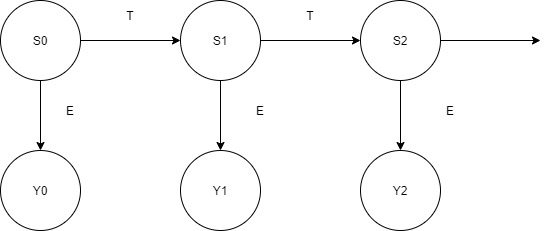
\includegraphics[width=0.5\textwidth]{images/hidden_markov_states.jpg}
\end{figure}

Imagine a model as in image \ref{hiddenMarkovStates}.
What is known: 
\begin{itemize}
    \item $p(y_t|s_t)$
    \item $p(s_t+1|s_t)$
\end{itemize}

From this we can deduce:
$$ p(s_0|y_0) = p(y_0|s_0) \frac{p(s_0)}{p(y_0)} $$
$$ p(s_1|y_0) = \Sigma_{s_0} p(s_1|s_0) p(s_0|y_0) $$
$$ p(y_1|y_0) = \Sigma_{s_0} \Sigma_{s_1} p(y_1|s_1) p(s_1|s_0) p(s_0|y_0) $$
Note that $ p(y_1|y_0) $ is not a function of either $s_0$ nor $s_1$.

\begin{equation}
    \begin{aligned}
        p(s_1|y_0, y_1) &= \frac{ p(y_1|s_1, y_0) p(s_1|y_0) }{ p(y_1|y_0) } \\
                        &= \frac{ p(y_1|s_1) p(s_1|y_0) }{ p(y_1|y_0) } \\
                        & \propto p(y_1|s_1) p(s_1|y_0) \text{ ... since $p(y_1|y_0)$ is not a function of $s$ }
    \end{aligned}
\end{equation}
(As reference, see the findings \ref{condPropLemmas}.)

More generally, we can write the \textbf{update-equation} as:
\begin{equation}
    p(s_t | \vec{y}_{[1..t]}) \propto p(y_t | s_t) p(s_t | \vec{y}_{[1..t-1]})
\end{equation}
... where $p(s_t | \vec{y}_{[1..t-1]})$ is the result of the last prediction equation.

With the \textbf{prediction-equation}:
\begin{equation}
    p(s_{t+1} | \vec{y}_{[1..t]} ) = \Sigma_{s_t} p(s_{t+1} | s_t) p(s_t | \vec{y}_{[1..t]}) )
\end{equation}
... where $ p(s_t | \vec{y}_{[1..t]}) $ is the result of the last update equation.

\begin{lstlisting}[language=python]
    states = ('Rainy', 'Sunny')
     
    observations = ('walk', 'shop', 'clean')
     
    start_prob = {'Rainy': 0.6, 'Sunny': 0.4}
     
    transition_prob = {
       'Rainy' : {'Rainy': 0.7, 'Sunny': 0.3},
       'Sunny' : {'Rainy': 0.4, 'Sunny': 0.6},
    }
     
    emission_prob = {
       'Rainy' : {'walk': 0.1, 'shop': 0.4, 'clean': 0.5},
       'Sunny' : {'walk': 0.6, 'shop': 0.3, 'clean': 0.1},
    }
    
    state_series = ['Rainy', 'Sunny', 'Sunny', 'Sunny', 'Rainy', 'Sunny', 'Rainy', 'Rainy', 'Sunny', 'Sunny', 'Sunny']
    emission_series = ['clean', 'walk', 'walk', 'shop', 'clean', 'shop', 'clean', 'clean', 'clean', 'shop', 'clean']
    
    
    def prediction(states, transition_prob, prob_St_Yt):
        prob_St1_Yt = {}
        for state1 in states:
            prob_St1_Yt[state1] = 0.0
            for state0 in states:
                prob_St1_Yt[state1] += transition_prob[state0][state1] * prob_St_Yt[state0]
        return prob_St1_Yt
    
    
    def update(states, emission, emission_prob, prob_St1_Yt):
        prob_St_Yt = {}
        for state in states:
            prob_St_Yt[state] = emission_prob[state][emission] * prob_St1_Yt[state]
        sm = sum(prob_St_Yt.values())
        for state in prob_St_Yt:
            prob_St_Yt[state] = prob_St_Yt[state] / sm
        return prob_St_Yt
    
            
    prob_St1_Yt = start_prob
    for t in range(10):
        emission = emission_series[t]
        prob_St_Yt = update(states, emission, emission_prob, prob_St1_Yt)
        prob_St1_Yt = prediction(states, transition_prob, prob_St_Yt)
\end{lstlisting}



\subsection{Tests}
This subsection is about what is the most common form of statistics in social sciences: tests.
Often, statistical tests work \emph{the wrong way round}. You have your hypothesis, like "these groups are different". Then you state the opposite, the \emph{null-hypothesis}. Then you determine how likely your data is under the null-hypothesis - the \emph{p-value}. And than you hope that the p-value is very low.

\paragraph{Students T-Test} compares two averages (means) and tells you if they are different from each other. The null hypothesis is that all samples come from the same distribution. That means that under $H_0$, the two means you obtained should be similar. So the interpretation goes like this: 
\begin{itemize}
    \item low p-value: the chance that your result would have happend under $H_0$ is low. It is very unlikely that the two means you have obtained actually come from the same distribution. 
    \item high p-value: It is quite possible that both your groups come from the same distribution. 
\end{itemize}
Note that there are two experimental setups that can use t-tests:
\begin{itemize}
    \item unpaired: you have two groups, with no person in both groups. Example: Test one group with medication and another with placebo. 
    \item paired: every person is first in the first and then in the second group. Example: test patients before and after treatment. 
\end{itemize}

\begin{figure}[H]
    \caption{Statistical test decision tree}
    \centering
    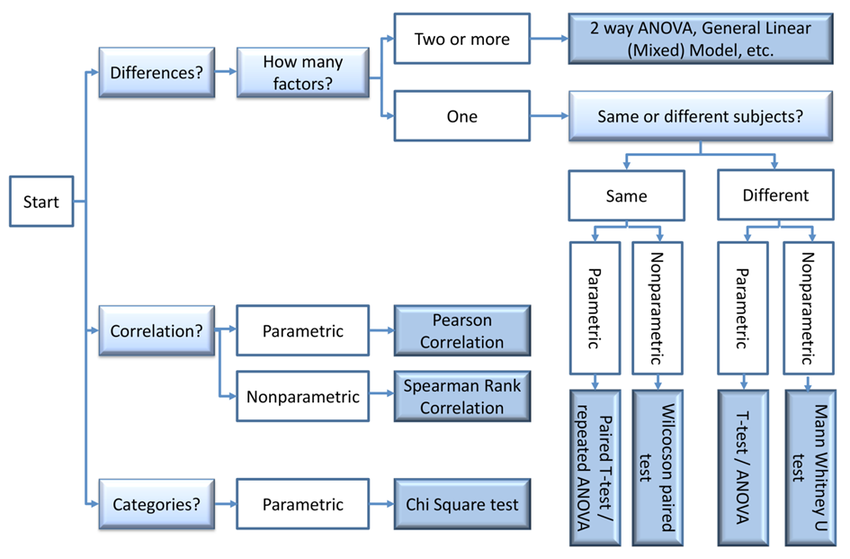
\includegraphics[width=0.7\linewidth]{images/statistical_test_decision_tree.png}
\end{figure}
